\section{Synchronous Neural Networks}
\label{sec:motivating-example}
\begin{figure}[b]
	\centering
	\begin{subfigure}[t]{0.4\textwidth}
		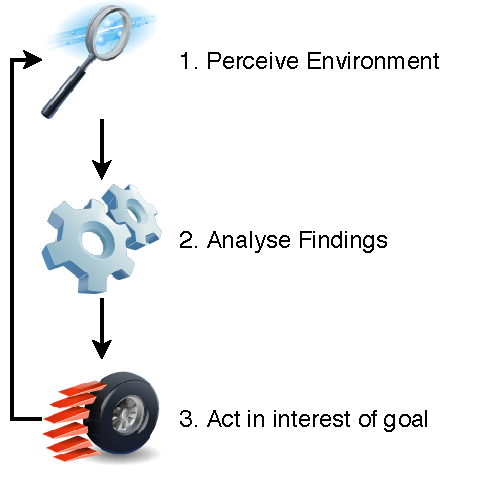
\includegraphics[width = \textwidth]{Content/fig/reactive-AI.pdf}
		\caption{Reactive \ac{AI}}
		\label{fig:reactive-ai}
	\end{subfigure}%
	\begin{subfigure}[t]{0.4\textwidth}
		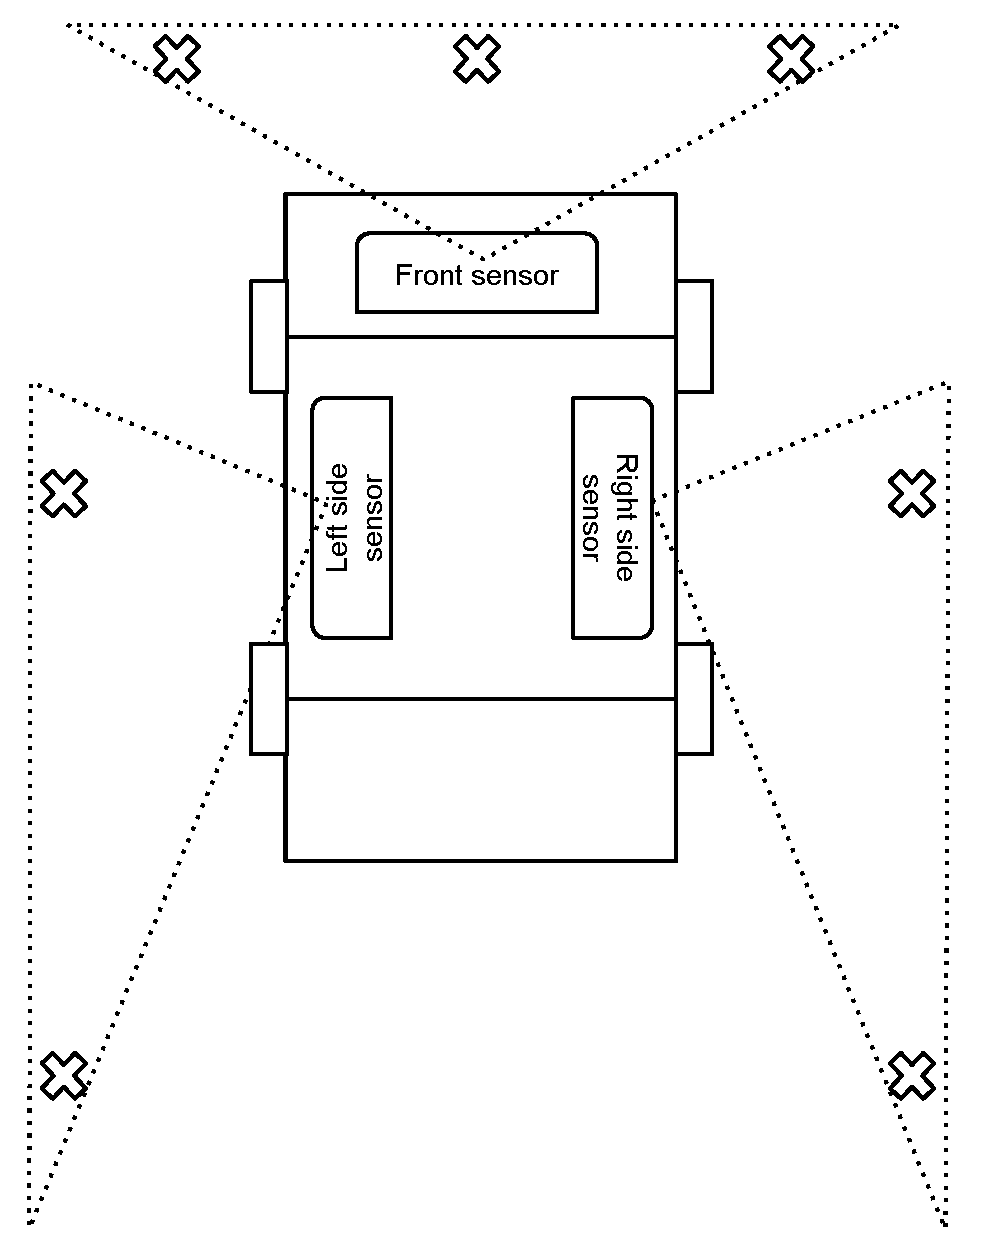
\includegraphics[width = \textwidth]{Content/fig/AutoVehicle.pdf}
		\captionsetup{justification=centering}
		\caption{Autonomous Vehicle Sensors}
		\label{fig:avimg}
	\end{subfigure}
	
	\caption{Reactive \texttt{AI-BRO}}
	\label{fig:reactive-aibro}
\end{figure}

Consider an autonomous vehicle, simplified for pedagogy, as shown in Figure~\ref{fig:avimg} as our motivating example.
The vehicle uses various sensors  to ``see'' the environment around it, while making \emph{lane changing decisions}. 
The sensor outputs are interpreted in order to make decisions based on the dynamic environment. 
The vehicle uses a number of sensors to detect objects in the environment around it. Based on these, it will decide when it needs to change lane
to the \emph{left} or \emph{right}, to \emph{continue} in the current lane, and when to \emph{stop} if necessary. 
The sensors consist of one frontal sensor and a sensor on each side.
The frontal sensor is simplified to detect three positions in front of the vehicle. The side sensors work similarly to the frontal sensor,
and each "see" two positions on each side of the vehicle. 
%Three \acp{ANN} are needed to analyse the sensor outputs in order to make driving decisions.

\acp{ANN} used in \ac{CPS} applications, such as lane changing, are used for decision making tasks 
needed by the controller. Such tasks operate periodically, being reactive in nature,
as shown in Figure~\ref{fig:reactive-ai}. We start by formalising \acp{SANN} using Definition~\ref{def:sann},
which are introduced by us. 

\begin{definition}
	\label{def:sann}
	A \acf{SANN} operates periodically, where the length of each period is 
	an integral multiple of the \emph{tick length} of a ``logical clock'' that \emph{tick}s. Tick length
	is a constant $\in \, \mathbb{R}^{>0}$.
\end{definition}

The periodic behaviour \acp{SANN}, as defined in Definition~\ref{def:sann}, are ideally implemented using the synchronous 
paradigm~\cite{benveniste2003synchronous} and we will use the Esterel programming language~\cite{berry2000foundations} 
to motivate the design of \acp{SANN}. Synchronous programs execute tick-by-tick and during a tick (also known as reaction) the
environment inputs are sampled, the overall system reaction is performed and finally emission of outputs are made. Thus, a tick encapsulates 
the atomicity of reactions, where inputs can happen only at the start of a tick, preventing race conditions arising due to environment 
non-determinism, which is widely prevalent in event triggered paradigms. A synchronous reaction is often represented as a composition of 
multiple, interacting \emph{threads} exhibiting \emph{logical concurrency}~\cite{benveniste2003synchronous}. 
These are usually \emph{compiled-away} to produce sequential code 
that avoid conventional race conditions widely prevalent in the asynchronous setting. Distributed compilation of threads, which is a much harder problem, over
multicore platforms is also well developed, though less widely used~\cite{yuan2011compiling}. The synchronous approach guarantees
key properties such as \emph{determinism} and \emph{reactivity}, which is ideal for AI-based CPS. This motivates 
our adoption of the this paradigm while designing \acp{SANN}.


%% add AI-BRO code here
\begin{figure}[htb]
	\begin{lstlisting}[caption={Esterel implementation of \texttt{AI-BRO}},label={lst:ai-bro}]
	module ai-bro:
	
	% data handling declarations -- omitted 
	
	% interface declarations
	input start, A, B, R;
	input fr1: integer, fr2: integer, fr3: integer;
	input s1: integer, s2: integer;
	input s3: integer, s4: integer;
	output O: integer;
	
	loop
	[
	await A;
	% run ANN A: interpret frontal scanner data
	present fr1 or fr2 or fr3 then
	call processFrontSensors()(?fr1, ?fr2, ?fr3);
	end present
	||
	await B;
	% run ANN B: interpret side scanner data
	present s1 or s2 or s3 or s4 then
	call processSideSensors()(?s1, ?s2, ?s3, ?s4);
	end present
	];
	
	% run ANN C: decide on best course of action 
	call makeDecision()();
	% fetch output action
	emit O(getAction());
	each R
	
	end module
	\end{lstlisting}
	%\label{fig:ai-bro}
\end{figure}

We have adapted Berry's well known ABRO example in Esterel~\cite{berry2000foundations} to develop our first example of 
\acp{SANN}. Being an adaptation of ABRO, we term our example, the AI-inspired ABRO, as \texttt{AI-BRO}, and present it in Listing~\ref{lst:ai-bro}.
The original ABRO example performs \emph{the emission of \texttt{O} when both inputs \texttt{A} and \texttt{B} 
	have happened. It resets and restarts this behaviour when the input \texttt{R} happens}. In our setting, the input 
\texttt{A} is used to control the processing of the frontal sensor, and the input \texttt{B} is used for the side sensors.
When both inputs have happened, we start the processing of the decision making network, which outputs the 
lane changing decision using the output \texttt{O}. \texttt{R} resets and restarts this behaviour.

The \texttt{AI-BRO} implementation in Esterel is done using an Esterel module called \texttt{ai-bro} shown in Listing~\ref{lst:ai-bro} on line~\#1.
A module is a basic programming unit in Esterel and the interface of the module consists of input and
output \emph{signals}. We have defined input signals \texttt{A, B, R}, which are \emph{pure signals}
i.e. these are Boolean in nature carrying a status --- either \emph{present / true} or \emph{absent / false} during a tick. The output signal 
\texttt{O} is valued and in addition to its status takes a value of type \texttt{integer}. The interface definitions appear in 
lines \#6-10. \ignore{While these defined signals have global scope, Esterel also has \emph{local signals} and \emph{local variables}, although these are not used in this 
	program. }% However, a local variable called \texttt{out} of type \texttt{integer} is defined on line \#10.
A variable, unlike a signal, has no status information. 

The main logic of the program is composed of two concurrent threads (denoted using the \texttt{||} operator)
that await external events \texttt{A, B} to happen. 
This task can be performed concurrently as these two inputs may happen either simultaneously in the same tick or 
in an interleaved manner in different ticks. Upon occurrence of the respective event, corresponding data processing 
is performed by the invocation of the appropriate \ac{ANN}, implemented as the C function \texttt{processFrontSensors()}
and \texttt{processSideSensors()}. Both these functions encapsulate pre-trained neural networks. Thus, when both events have 
happened and both networks have executed, the two concurrent threads are terminated. The two threads are also grouped using the 
grouping operators (denoted by \texttt{[ ]}), which are put in sequence using the sequence operator (denoted by the ``\texttt;''). %,with the statements starting from line \#24. 
Thus the third neural network, called \texttt{makeDecision()},
can trigger only after the data from both the front and side sensors have been processed. 
The output of this decision is subsequently emitted through the valued signal \texttt{O}, on line \#30, which will indicate the chosen lane changing action.

Finally, the main logic is enclosed in a \texttt{loop..each R} construct. This is a \emph{preemption construct} that preempts and restarts the 
loop on every \texttt{R} input, maintaining reactive behaviour with every reset.
This will happen after each lane changing decision.

\ignore{The first \ac{SANN} takes input from the frontal sensor, i.e. it receives three integer inputs (either 1 or -1). 
	This \ac{SANN} the outputs the suggested course of action based off of these inputs: stop, turn left/right or continue.  
	The second \ac{SANN} takes input from both side sensors, i.e. it receives four integer inputs (either 1 or -1). 
	This \ac{SANN} returns a simplified version of whether or not is it safe for the vehicle to move in either direction.
	The last \ac{SANN} takes in the outputs of the first and second \acp{SANN} and decides on the best course of action
	for the vehicle based on those inputs: stop, turn left/right or continue.}

The \texttt{AI-BRO} example illustrates several features of \acp{SANN}. (1) We are able to create \acp{ANN} that trigger periodically (analogous
to \acp{RNN}) and we can control the timing of these invocations, and (2) Within each period, we can precisely synchronise the 
execution of different \acp{ANN} i.e. the sensor processing \acp{ANN} are synchronised with the external inputs 
\texttt{A, B} while the decision making \ac{ANN} is executed immediately after the first two \acp{ANN} have finished. 
To the best of our knowledge, such precise synchronisation mechanisms are lacking in existing literature on \acp{ANN}.
More importantly, a side effect of the Esterel implementation is that the resultant \ac{ANN} compositions are 
either rejected by the compiler as \emph{non-causal} or compiled into a \emph{causal} implementation that is guaranteed to be
\emph{deterministic} and \emph{reactive}~\cite{benveniste2003synchronous}.

\ignore{the running of \acp{SANN} concurrently and consecutively. If signals A and B are high on the same tick, then both sensor \acp{SANN} will run at the same time. The decision \ac{SANN} will always run after both of the sensor \acp{SANN}. Since these are implemented in Esterel, the system remains causal, deterministic, bounded and, most importantly, time predictable. WCET analysis can be run on AIBRO, with results that are well within the acceptable prediction range.}


\ignore{
	\begin{lemma}
		\label{lemma1}
		The AI-ABRO implementation in Listing~\ref{lst:ai-bro} is an instance of \ac{SANN} defined using Definition~\ref{def:sann}.
	\end{lemma}
}

\begin{prop}
	\label{lemma1}
	The AI-ABRO implementation in Listing~\ref{lst:ai-bro} is an instance of \ac{SANN} defined using Definition~\ref{def:sann}.
\end{prop}

\begin{proof}
	The proof of this trivially follows from the fact that this program is compiled to a single \texttt{tick()} function by the 
	Esterel compiler, where the concurrency is compiled away. Thus, during any tick, we can have a combination of neural networks 
	executing that range from just one network to up to three networks. Assuming that we can execute this program with a fixed tick length 
	(elaborated in section~\ref{sec:wcrt}), the overall period of any network is at most 1-tick. 
\end{proof}
